% ============================================================
%  EduReach — Progress Report & Budget Review
%  Period: May 2026
%  Compiled with pdflatex (upload logo.jpeg alongside this file in Overleaf)
% ============================================================
\documentclass[12pt,a4paper]{article}

% ── packages ────────────────────────────────────────────────
\usepackage[a4paper, top=2.5cm, bottom=2.5cm, left=2.8cm, right=2.8cm]{geometry}
\usepackage{graphicx}
\usepackage{xcolor}
\usepackage{booktabs}
\usepackage{tabularx}
\usepackage{longtable}
\usepackage{array}
\usepackage{enumitem}
\usepackage{tikz}
\usepackage{pgfplots}
\usepackage{pgf-pie}
\pgfplotsset{compat=1.18}
\usepackage{mdframed}
\usepackage{fancyhdr}
\usepackage{titlesec}
\usepackage{parskip}
\usepackage{hyperref}
\usepackage{fontawesome5}
\usepackage{multirow}
\usepackage{colortbl}
\usepackage{amsmath}

% ── brand colours ────────────────────────────────────────────
\definecolor{indigo}{HTML}{4F46E5}
\definecolor{indigodark}{HTML}{3730A3}
\definecolor{indigolight}{HTML}{EEF2FF}
\definecolor{slate}{HTML}{475569}
\definecolor{slatelight}{HTML}{F8FAFC}
\definecolor{emerald}{HTML}{059669}
\definecolor{amber}{HTML}{D97706}
\definecolor{rose}{HTML}{E11D48}
\definecolor{rowgray}{HTML}{F1F5F9}

\hypersetup{colorlinks=true, linkcolor=indigo, urlcolor=indigo}

% ── section styling ──────────────────────────────────────────
\titleformat{\section}{\large\bfseries\color{indigodark}}{}{0em}{}[\vspace{-4pt}\rule{\linewidth}{1.5pt}]
\titleformat{\subsection}{\normalsize\bfseries\color{slate}}{}{0em}{}

% ── header / footer ──────────────────────────────────────────
\pagestyle{fancy}
\fancyhf{}
\fancyhead[L]{\small\color{slate}\textbf{EduReach} \textbar\ Progress Report}
\fancyhead[R]{\small\color{slate}May 2026 \textbar\ Strictly Internal}
\fancyfoot[C]{\small\color{slate}\thepage}
\renewcommand{\headrulewidth}{0.4pt}

% ── helper: coloured badge ────────────────────────────────────
\newcommand{\badge}[2]{%
  \colorbox{#1}{\small\color{white}\textbf{\ #2\ }}%
}
\newcommand{\done}{\badge{emerald}{DONE}}
\newcommand{\inprog}{\badge{amber}{IN PROGRESS}}
\newcommand{\notyet}{\badge{rose}{NOT YET}}

% ── thin rule ────────────────────────────────────────────────
\newcommand{\hrulesmall}{\vspace{2pt}\noindent\textcolor{indigolight}{\rule{\linewidth}{0.6pt}}\vspace{4pt}}

% ============================================================
\begin{document}

% ──────────────────────────────────────────────────────────────
%  COVER PAGE
% ──────────────────────────────────────────────────────────────
\begin{titlepage}
  \pagecolor{indigodark}
  \color{white}
  \centering
  \vspace*{3cm}

  % Logo — upload logo.jpeg next to this .tex file in Overleaf
  \IfFileExists{logo.jpeg}{%
    
\includegraphics[width=4cm]{logo.jpeg}\\[0.6cm]
  }{%
    {\Huge\bfseries\color{white} EduReach}\\[0.6cm]
  }

  {\huge\bfseries Progress Report \& Budget Review}\\[0.4cm]
  {\large May 2026}\\[0.8cm]

  \hrulesmall

  \vspace{0.6cm}
  {\normalsize
    \begin{tabular}{rl}
      \textbf{Company:}   & EduReach \\[4pt]
      \textbf{Sector:}    & EdTech / AI-Powered Learning \\[4pt]
      \textbf{Market:}    & African \& Developing World \\[4pt]
      \textbf{Stage:}     & MVP — Post-Launch \\[4pt]
      \textbf{Website:}   & \texttt{https://edureach.site} \\[4pt]
      \textbf{Team:}      & Dalton Omondi (Co-founder) \\[4pt]
                          & Mary Syokau (Co-founder) \\
    \end{tabular}
  }

  \vfill
  {\small\color{white!70} Strictly Internal Document — Not for External Distribution}
\end{titlepage}
\pagecolor{white}\color{black}

% ──────────────────────────────────────────────────────────────
\tableofcontents
\newpage

% ============================================================
\section{Executive Summary}

EduReach is a mobile-first, AI-driven learning platform built natively for the African market.
We solve the problem of passive online learning by transforming existing YouTube content into
structured, interactive courses complete with AI-generated quizzes, personal AI tutors, and
social study groups. Teams can participate in graded assessments, compete, and achieve rankings.

By integrating with local mobile-money networks (M-Pesa, Paystack), EduReach removes the
geographical and financial barriers of Western learning platforms. We provide a scalable,
creator-friendly ecosystem that turns video consumption into genuine, measurable education.

\begin{mdframed}[linecolor=indigo, linewidth=1.5pt, leftmargin=0pt, innerleftmargin=12pt,
  innertopmargin=8pt, innerbottommargin=8pt, backgroundcolor=indigolight]
\textbf{Snapshot as at May 2026}\\[4pt]
\begin{tabular}{llll}
  \faUsers\ \textbf{117} total users
  & \faCheckCircle\ \textbf{33\%} active
  & \faDollarSign\ \textbf{0} paying
  & \faCode\ MVP: \textbf{Complete} \\
\end{tabular}
\end{mdframed}

% ============================================================
\section{Progress Against Goals}

\subsection{Strategic Goals (Set at Launch)}

\begin{tabularx}{\linewidth}{>{\bfseries}p{0.45\linewidth} X c}
\toprule
\textbf{Goal} & \textbf{Status} & \textbf{Achieved?} \\
\midrule
\rowcolor{rowgray}
Onboard at least 2,500 users & 117 registered (4.7\% of target). Growth has been
organic with no paid acquisition yet. & \notyet \\[4pt]
At least 350 active users & $\approx$39 active (33\% of 117; 11\% of target).
Active is defined as having used the platform after sign-up. & \notyet \\[4pt]
\rowcolor{rowgray}
At least 50 paying users & 0 paying users. Monetisation has not yet been activated.
A pricing page and billing system are live and ready. & \notyet \\[4pt]
Sign MOU with African Olympiad Academy & Discussions are ongoing.
The platform now contains high-quality olympiad-style content as a proof point. & \inprog \\
\bottomrule
\end{tabularx}

\vspace{6pt}
\textbf{Note on user growth:} 67\% of registered users signed up and became inactive.
The newly implemented 14-day guest trial (no account required) is designed to
address this directly — users experience value before committing to registration.

\subsection{Sprint Goals (This Period)}

\begin{tabularx}{\linewidth}{>{\bfseries}p{0.48\linewidth} X c}
\toprule
\textbf{Goal} & \textbf{Notes} & \textbf{Status} \\
\midrule
\rowcolor{rowgray}
Clear \& communicative landing page & Landing page redesigned: general-purpose
language, new ``Try it free — no account needed'' CTA, updated trust signals. & \done \\[4pt]
Bring a potential first paying customer & Outreach ongoing. Billing page and
payment flows are fully live. & \inprog \\[4pt]
\rowcolor{rowgray}
Resolve recurring bugs & Mobile overflow, answer input wrap, Google Sign-In,
API interceptors, assessment pagination, tab navigation — all resolved. & \done \\[4pt]
Onboard Kenyan IMO team into the platform & Olympiad content seeded.
Direct outreach not yet completed. & \inprog \\
\bottomrule
\end{tabularx}

% ============================================================
\section{Technical Achievements This Period}

The following features and fixes were shipped to production during this period:

\subsection{New Features}
\begin{itemize}[leftmargin=1.4em, itemsep=3pt]
  \item \textbf{Lazy authentication / guest trial:}
        New visitors get 14 days of full platform access with no account required.
        At 14 days, a forced sign-up prompt appears. Write actions (create content,
        join study groups) are blocked with a plain explanation and sign-up CTA.
  \item \textbf{Olympiad assessment seeder:}
        Seeded mixed-subfield olympiad-style papers across Mathematics, Physics,
        Chemistry, and Biology — each with varied question types.
  \item \textbf{Pop-out AI chat assistant:}
        Floating AI panel available on all pages, toggleable from the learning session.
  \item \textbf{Relevance ranking \& EduReach personalisation:}
        Dashboard content is ranked by learner type and stated interests.
  \item \textbf{Study group challenge picker:}
        Searchable assessment selector in study group challenge creation,
        with type filter tabs (Quiz / Exam) and live search.
  \item \textbf{Deferred AI marking:}
        Assessment submission now only saves answers.
        A ``Mark with AI'' button appears separately — users choose when to see results.
        This resolves confusion reported by students who could not pivot after seeing
        immediate feedback.
  \item \textbf{Image-based answer support:}
        Students can photograph handwritten work and submit as an answer image.
        The AI grader is wired to grade from uploaded images.
\end{itemize}

\subsection{Bug Fixes \& UX Improvements}
\begin{itemize}[leftmargin=1.4em, itemsep=3pt]
  \item Mobile horizontal overflow resolved across Assessments, Landing Page,
        Learning Session, and MathMarkdown (KaTeX equations).
  \item Study groups dashboard tabs now scroll horizontally on mobile —
        the Events and Invites tabs were previously unreachable on phones.
  \item Answer input fields converted from single-line \texttt{<input>} to
        auto-growing \texttt{<textarea>} with word wrap.
  \item Google Sign-In switched from passive One Tap (\texttt{prompt()})
        to explicit button flow (\texttt{renderButton()}) — resolves browser suppression.
  \item ErrorBoundary now shows a clean user message in production instead of
        raw JavaScript error text.
  \item API interceptors updated: 401 errors during guest mode fail silently
        instead of triggering the session-expired redirect.
  \item Microeconomics assessment content completely replaced:
        6 assessments now contain 10 real university-level MCQ questions each,
        with options, correct answers, and explanations.
  \item Assessment list now returns all records in one response (was capped at 20).
  \item Subject filter dropdown removed from assessments page (was causing confusion).
\end{itemize}

% ============================================================
\section{User Metrics}

\begin{center}
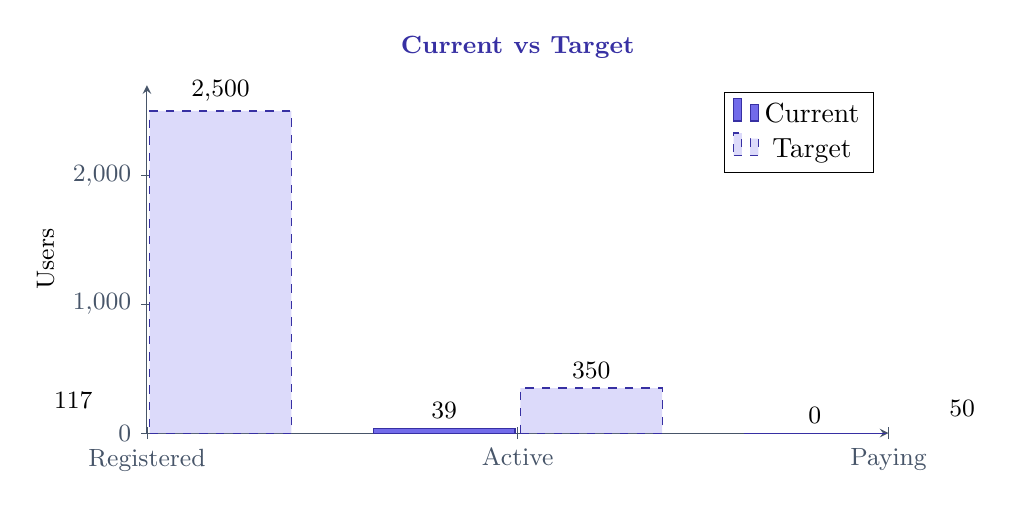
\begin{tikzpicture}
\begin{axis}[
  ybar,
  bar width=1.8cm,
  width=11cm, height=6cm,
  symbolic x coords={Registered, Active, Paying},
  xtick=data,
  ymin=0, ymax=2700,
  ylabel={Users},
  ylabel style={font=\small},
  xlabel style={font=\small},
  nodes near coords,
  nodes near coords style={font=\small\bfseries},
  axis lines=left,
  axis line style={color=slate},
  tick style={color=slate},
  xticklabel style={font=\small\color{slate}},
  yticklabel style={font=\small\color{slate}},
  title={Current vs Target},
  title style={font=\small\bfseries\color{indigodark}},
]
\addplot[fill=indigo!80, draw=indigodark] coordinates {(Registered,117) (Active,39) (Paying,0)};
\addplot[fill=indigo!20, draw=indigodark, dashed] coordinates {(Registered,2500) (Active,350) (Paying,50)};
\legend{Current, Target}
\end{axis}
\end{tikzpicture}
\end{center}

\begin{tabularx}{\linewidth}{X r r r}
\toprule
\textbf{Metric} & \textbf{Current} & \textbf{Target} & \textbf{\% of Target} \\
\midrule
\rowcolor{rowgray}
Total registered users & 117 & 2,500 & 4.7\% \\
Active users & $\approx$39 & 350 & 11.1\% \\
\rowcolor{rowgray}
Paying users & 0 & 50 & 0\% \\
Activation rate (signed up \& stayed active) & 33\% & 70\%+ & — \\
\bottomrule
\end{tabularx}

\vspace{6pt}
\textbf{Observation:} The 67\% dormancy rate is the most critical metric to address.
Root cause: users created accounts before experiencing product value.
The guest trial directly addresses this by delivering value first.

% ============================================================
\section{Financial Report}

\subsection{This Period — Expenditure}

All amounts in Kenyan Shillings (KES). USD converted at 130 KES/USD.

\begin{tabularx}{\linewidth}{X r r l}
\toprule
\textbf{Item} & \textbf{Amount (KES)} & \textbf{Amount (USD)} & \textbf{Notes} \\
\midrule
\rowcolor{rowgray}
Render (hosting — migrated away) & 1,808.20 & $\approx$13.91 &
  Render had RAM limits; migrated to Contabo for better cost/performance. \\
Claude Pro (AI subscription) & 3,175.19 & $\approx$24.42 &
  Used for product development, content generation, and code assistance. \\
\rowcolor{rowgray}
Contabo VPS (new hosting) & 1,708.66 & $\approx$13.14 &
  KES 250/month cheaper than Render for the same spec; better long-term option. \\
OpenRouter API credits & 1,300.00 & $\approx$10.00 &
  AI inference credits for platform AI features (quiz generation, grading, tutoring). \\
\midrule
\textbf{Total Expenditure} & \textbf{7,992.05} & \textbf{$\approx$61.48} & \\
\bottomrule
\end{tabularx}

\subsection{Cash Position}

\begin{tabularx}{\linewidth}{X r}
\toprule
\textbf{Item} & \textbf{Amount (KES)} \\
\midrule
\rowcolor{rowgray}
Opening cash & 11,138.40 \\
Total expenditure this period & (7,992.05) \\
\midrule
\textbf{Closing cash / Available balance} & \textbf{3,146.35} \\
\bottomrule
\end{tabularx}

\subsection{Expenditure Breakdown}

\begin{center}
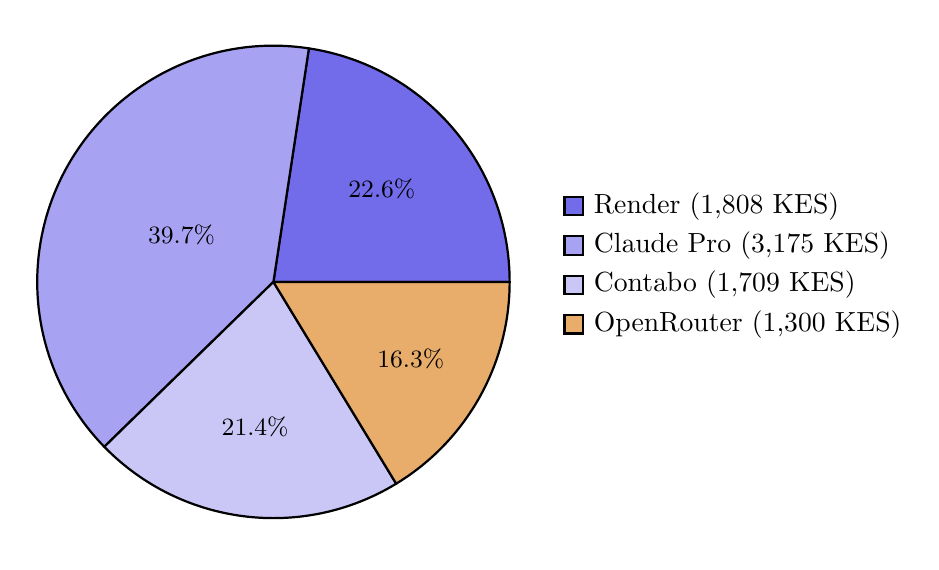
\begin{tikzpicture}
\pie[
  radius=3,
  color={indigo!80, indigo!50, indigo!30, amber!60},
  text=legend,
  before number=\small,
  after number=\%,
]
{22.6/{Render (1,808 KES)},
 39.7/{Claude Pro (3,175 KES)},
 21.4/{Contabo (1,709 KES)},
 16.3/{OpenRouter (1,300 KES)}}
\end{tikzpicture}
\end{center}

\subsection{Justification of Expenditure}

\textbf{Why Render was replaced by Contabo:}
Render's free and lower tiers impose RAM limits that caused the backend
to crash under load. Contabo provides a dedicated VPS with 4 GB RAM
at a lower monthly cost — a necessary infrastructure upgrade for reliability
as user numbers grow.

\textbf{Why Claude Pro is the largest single expense:}
Claude Pro was used intensively this period for full-stack product development
(all features described in Section 3), content generation (olympiad papers,
microeconomics question banks), and the co-founder agreement.
This will reduce significantly once the platform reaches feature-stability.

\textbf{OpenRouter credits:}
Required for the platform's live AI features — AI quiz generation, AI grading,
and the AI tutor. These are direct product costs, not development costs.

% ============================================================
\section{Next Month Budget Projection}

\subsection{Known Costs (Committed)}

\begin{tabularx}{\linewidth}{X r r l}
\toprule
\textbf{Item} & \textbf{USD} & \textbf{KES (@ 130)} & \textbf{Notes} \\
\midrule
\rowcolor{rowgray}
Contabo VPS & 5.40 & 702 & Monthly server hosting \\
OpenRouter API credits & 10.00 & 1,300 & AI features — quiz generation, grading \\
\rowcolor{rowgray}
Utilities \& printing & — & 1,000 & Office costs, printed materials for outreach \\
\midrule
\textbf{Committed total} & \textbf{15.40} & \textbf{3,002} & \\
\bottomrule
\end{tabularx}

\subsection{Contingent Cost}

\begin{tabularx}{\linewidth}{X r r l}
\toprule
\textbf{Item} & \textbf{USD} & \textbf{KES (@ 130)} & \textbf{Scenario} \\
\midrule
\rowcolor{rowgray}
Claude Pro (if renewed) & 20.00 & 2,600 & Only if intensive development continues \\
\bottomrule
\end{tabularx}

\subsection{Cash Projection}

\begin{tabularx}{\linewidth}{X r}
\toprule
\textbf{Scenario} & \textbf{Closing Cash (KES)} \\
\midrule
\rowcolor{rowgray}
Without Claude Pro renewal & 3,146.35 − 3,002 = \textbf{144.35} \\
With Claude Pro renewal & 3,146.35 − 5,602 = \textbf{(2,455.65) — shortfall} \\
\bottomrule
\end{tabularx}

\begin{mdframed}[linecolor=rose, linewidth=1.5pt, innerleftmargin=12pt,
  innertopmargin=8pt, innerbottommargin=8pt, backgroundcolor=rose!5]
\textbf{\color{rose}\faExclamationTriangle\ Cash Warning}\\[4pt]
Even without Claude Pro, only KES 144 remains after next month's committed costs.
This leaves \textbf{zero buffer} for unexpected expenses, outreach costs, or new
infrastructure needs. We need additional capital injection before end of May.
\end{mdframed}

\subsection{Recommendations}

\begin{enumerate}[leftmargin=1.6em, itemsep=4pt]
  \item \textbf{Reduce AI development costs:} Now that the platform is feature-stable,
        Claude Pro usage will drop. Consider switching to the API (pay-per-use)
        rather than a flat Pro subscription.
  \item \textbf{Pursue first paying customer urgently:} Even one school paying
        KES 2,000–5,000/month covers most recurring costs.
  \item \textbf{Activate monetisation:} The billing page, Stripe/M-Pesa integration,
        and pricing tiers are all live. Enable the Free → Paid upgrade funnel now.
  \item \textbf{Seek a small cash injection:} KES 10,000–15,000 provides a 3-month
        runway buffer and funds outreach materials / demo events.
\end{enumerate}

% ============================================================
\section{Roadmap — Next 30 Days}

\begin{tabularx}{\linewidth}{>{\bfseries}p{0.38\linewidth} X p{0.15\linewidth}}
\toprule
\textbf{Priority} & \textbf{Action} & \textbf{Owner} \\
\midrule
\rowcolor{rowgray}
1 — Critical & Secure first paying customer (individual or institution) & Dalton \\
2 — Critical & Activate the monetisation funnel — run a sign-up and prompt to upgrade & Both \\
\rowcolor{rowgray}
3 — High & MOU with African Olympiad Academy — schedule formal meeting & Dalton \\
4 — High & Outreach to Kenyan IMO team — demo session on the platform & Both \\
\rowcolor{rowgray}
5 — Medium & Post-signup plan selection modal (pick a plan after account creation) & Mary \\
6 — Medium & Personalisation prompts via notification system & Mary \\
\rowcolor{rowgray}
7 — Low & Launch a simple referral programme to drive organic user growth & Both \\
\bottomrule
\end{tabularx}

% ============================================================
\section{Key Risks}

\begin{tabularx}{\linewidth}{>{\bfseries}p{0.3\linewidth} X p{0.18\linewidth}}
\toprule
\textbf{Risk} & \textbf{Detail} & \textbf{Mitigation} \\
\midrule
\rowcolor{rowgray}
Cash runway & $<$ KES 200 buffer after next month's costs & First customer / injection \\
Zero revenue & Platform is live and capable; monetisation not yet active &
  Activate billing urgently \\
\rowcolor{rowgray}
High dormancy rate & 67\% of sign-ups never returned &
  Guest trial removes sign-up friction \\
No institutional anchor & MOU pending — credibility gap for school outreach &
  African Olympiad MOU priority \\
\rowcolor{rowgray}
Single-server risk & One Contabo VPS with no redundancy &
  Acceptable at current scale; review at 1k users \\
\bottomrule
\end{tabularx}

% ============================================================
\section{Platform Overview (For Demos)}

\begin{mdframed}[linecolor=indigo, linewidth=1pt, innerleftmargin=12pt,
  innertopmargin=8pt, innerbottommargin=8pt, backgroundcolor=indigolight]
\textbf{What EduReach does — in one paragraph:}\\[4pt]
EduReach takes YouTube educational videos and wraps them in structure, accountability,
and AI. A student opens a YouTube link, our platform adds chapter structure, generates
quizzes automatically, lets the student ask the AI tutor questions mid-lesson, and
records their progress. Schools can create graded assessments with AI marking, run
olympiad-style competitions, and track every student's performance through an analytics
dashboard. All of this works on mobile, costs a fraction of Western alternatives,
and accepts M-Pesa payments.
\end{mdframed}

\vspace{0.5cm}
\begin{tabularx}{\linewidth}{>{\bfseries}X X}
\toprule
\textbf{Feature} & \textbf{Status} \\
\midrule
\rowcolor{rowgray}
YouTube → Structured Course converter & \done \\
AI Quiz Generator (from video / text / PDF) & \done \\
\rowcolor{rowgray}
AI Tutor (per-lesson chat) & \done \\
Graded Assessments with AI Marking & \done \\
\rowcolor{rowgray}
Study Groups with Challenges \& Leaderboards & \done \\
Olympiad-style Exam Papers & \done \\
\rowcolor{rowgray}
M-Pesa / Paystack Payment Integration & \done \\
Mobile-First PWA (installable on Android) & \done \\
\rowcolor{rowgray}
14-Day Guest Trial (no account needed) & \done \\
Analytics Dashboard for Educators & \done \\
\rowcolor{rowgray}
Image-Based Answer Submission & \done \\
Post-Signup Plan Selection & \inprog \\
\bottomrule
\end{tabularx}

% ──────────────────────────────────────────────────────────────
\vfill
\begin{center}
\small\color{slate}
EduReach \textbar\ \texttt{edureach.site} \textbar\ \texttt{edu.reach.co@gmail.com}\\
Dalton Omondi \& Mary Syokau \textbar\ Nairobi, Kenya \textbar\ May 2026\\[4pt]
\textit{This document is strictly internal. Not for external distribution without consent of both co-founders.}
\end{center}

\end{document}
